\documentclass[aspectratio=169, xcolor={usenames,svgnames,dvipsnames}]{beamer}
\usepackage[utf8]{inputenc}
\usepackage[T1]{fontenc}
\usepackage{graphicx}
\usepackage{grffile}
\usepackage{cancel}
\usepackage{longtable}
\usepackage{wrapfig}
\usepackage{rotating}
\usepackage[normalem]{ulem}
\usepackage{amsmath}
\usepackage{textcomp}
\usepackage{amssymb}
\usepackage{capt-of}
\usepackage{hyperref}
\usepackage{color}
\usepackage{listings}
\usepackage{mathpazo}
\usepackage{gensymb}
\usepackage{amsmath}
\usepackage{diffcoeff}
\usepackage{steinmetz}
\usepackage{mathtools}
\bibliographystyle{plain}
\usepackage{siunitx}
\sisetup{output-decimal-marker={,}, retain-unity-mantissa = false}
\DeclareSIUnit{\watthour}{Wh}
\hypersetup{colorlinks=true, linkcolor=Blue, urlcolor=Blue}
\renewcommand{\thefootnote}{\fnsymbol{footnote}}
\newcommand{\laplace}[1]{\mathbf{#1}(\mathbf{s})}
\newcommand{\slp}{\mathbf{s}}
\newcommand{\fasor}[1]{\mathbf{#1}(\omega)}
%\newcommand{\arctan}{\mathrm{atan}}
\parskip=5pt
\usetheme{Boadilla}
\usecolortheme{rose}
\usefonttheme{serif}
\author{Ana Fernández-Guillamón}
\date{}
\title{Circuitos de Corriente Alterna}
\subtitle{Teoría de Circuitos}
\setbeamercolor{alerted text}{fg=blue!50!black} \setbeamerfont{alerted text}{series=\bfseries}
\makeatletter
\patchcmd{\beamer@sectionintoc}{\vskip1.5em}{\vskip1em}{}{}
\makeatother
%\AtBeginSection[]{\begin{frame}[plain]\tableofcontents[currentsection,hideallsubsections]\end{frame}}
%\AtBeginSubsection[]{\begin{frame}[plain]\tableofcontents[currentsubsection,sectionstyle=show/shaded,subsectionstyle=show/shaded/hide]\end{frame}}
\beamertemplatenavigationsymbolsempty
\setbeamertemplate{footline}[frame number]
\setbeamertemplate{itemize items}[triangle]
\setbeamertemplate{enumerate items}[circle]
\setbeamertemplate{section in toc}[circle]
\setbeamertemplate{subsection in toc}[circle]
\setbeamertemplate{blocks}[shadow=false]

\usepackage{multicol}
\AtBeginSubsection
{\begin{frame}[plain]
\begin{multicols}{2}
\tableofcontents[currentsubsection,sectionstyle=show/shaded,subsectionstyle=show/shaded/hide]
\end{multicols}
\end{frame}}
\AtBeginSection[]
{\begin{frame}[plain]
\begin{multicols}{2}
\tableofcontents[currentsection,hideallsubsections]
\end{multicols}
\end{frame}}


\begin{document}

\maketitle

\section{Formas de onda periódicas}

\begin{frame}{Formas de onda periódicas}

\begin{equation*}
    y(t)=y(t+T)=y(t+n\cdot T)
\end{equation*}

\begin{itemize}
		\item \alert{Período ($T$)}: intervalo de tiempo a partir del cual se repite la forma de onda [s]
		\item \alert{Frecuencia ($f$)}: número de veces que se repite la onda por unidad de tiempo [Hz]:
		\begin{equation*}
			f = \dfrac{1}{T}
		\end{equation*}
		\item \alert{Valor instantáneo ($y(t)$)}: valor que toma la forma de onda en un instante de tiempo 
		\item \alert{Valores de pico ($Y_{max}$, $Y_{min}$)}: valores máximo y mínimo que toma la forma de onda:
		\begin{equation*}
			Y_{max} = \max(f(t)); \qquad Y_{min} = \min(f(t))
		\end{equation*}
		\item \alert{Valor pico a pico ($Y_{PP}$)}: diferencia (en valor absoluto) entre los valores de pico considerados con signo: 
		\begin{equation*}
			Y_{PP}=|Y_{max} - Y_{min}|
		\end{equation*}
		\end{itemize}
		\end{frame}
		
		\begin{frame}{Forma de onda periódicas}
		\begin{itemize}
		\item \alert{Valor medio ($Y_m$)}: media aritmética de los valores instantáneos que toma la función en un periodo (semi-periodo o cuarto de periodo): 
		\begin{equation*}
			\boxed{Y_m=\frac{1}{T}\int_{a}^{a+T}y(t)\, dt}
		\end{equation*}
		\item \textbf{Valor eficaz ($Y_{ef}$)}: raíz cuadrada de la media de los cuadrados de los valores que toma la función en un periodo
		\begin{equation*}
			\boxed{Y_{ef} = \sqrt{\frac{1}{T}\cdot\int_{a}^{a+T}y^{2}(t)\, dt}}
		\end{equation*}
	\end{itemize}
\end{frame}

\subsection{Función sinusoidal}

\begin{frame}{Función sinusoidal}
\begin{center}
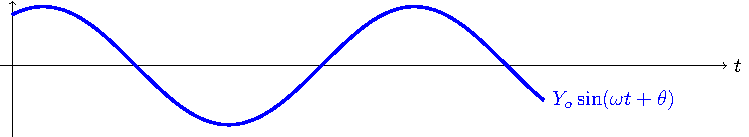
\includegraphics[width=.9\linewidth]{../figs/sin.pdf}
\end{center}

\begin{itemize}
\item \(Y_{max}\) valor máximo de la onda

\item \(\omega=2\cdot\pi\cdot f\): pulsación [rad/s]

\item \(f=\frac{\omega}{2\cdot\pi}\): frecuencia [Hz]

\item $T=\frac{1}{T}$: periodo de la onda [s]

\item \(\theta\): fase [rad] (o [$\si{}{\degree}$])
\end{itemize}
\end{frame}


\begin{frame}{Función sinusoidal}{Fase}
\begin{center}
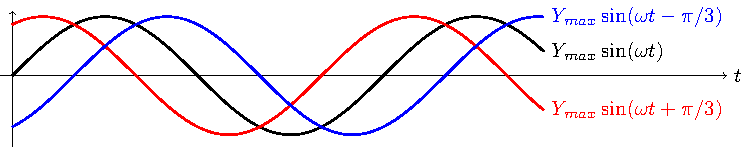
\includegraphics[width=.9\linewidth]{../figs/desfase.pdf}
\end{center}

\begin{itemize}
\item Fase:
\begin{itemize}
\item Es el argumento de la onda para $t=0$

\item Tomando una onda como referencia, si la fase es 0º, se dice que
está \alert{en fase} con la de referencia

\item Si la fase es positiva, se dice que la onda \alert{se adelanta} a la referencia

\item Si la fase es negativa, se dice que la onda \alert{se retrasa} a la referencia
\end{itemize}
\end{itemize}
\end{frame}

\begin{frame}{Función sinusoidal}{Valor medio y valor eficaz}
\begin{block}{Valor medio}
\[
Y_m=\frac{1}{T}\int_{0}^{T}y(t)\, dt = 0
\]

\[
Y_m=\frac{1}{T/2}\int_{0}^{T/2}Y_{max}\cdot\sin(\omega \cdot t)\, dt=\boxed{\dfrac{2\cdot Y_{max}}{\pi}\approx 0.637\cdot Y_{max}}
\]
\end{block}
\begin{block}{Valor eficaz}
\[
Y = \sqrt{\frac{1}{T}\cdot\int_{0}^{T}y^{2}(t)\, dt}
\]

\[
Y=\sqrt{\frac{1}{T}\cdot\int_{0}^{T}\left(Y_{max}\cdot\sin(\omega\cdot t)\right)^{2}dt}=\boxed{\frac{Y_{max}}{\sqrt{2}}}
\]
\end{block}
\end{frame}

\subsection{Cálculo fasorial}

\begin{frame}{Cálculo fasorial}{Representación fasorial}
\begin{itemize}
\item Un fasor es un \alert{vector giratorio} que gira en sentido contrario a las agujas del reloj a velocidad $\omega$: \href{https://www.youtube.com/watch?v=9U8_XfBtFrY&ab_channel=Ponuningenieroentuvida}{vídeo}
\item El \alert{módulo} del fasor es el \alert{valor eficaz}; el \alert{argumento} es la \alert{fase}
\item Descartamos pulsación: No se puede emplear cuando hay frecuencias diferentes en un mismo circuito
\end{itemize}

\begin{columns}
\begin{column}{0.65\columnwidth}
\begin{align*}
\text{Forma polar: }& \overline{Y} = Y_{ef}\phase{\theta}\\
\text{Forma binómica: }& \overline{Y} = Y_{ef}\cdot(\cos(\theta)+\mathrm{j}\cdot\sin(\theta))
\end{align*}

\begin{block}{Consideraciones}
 \begin{itemize}
     \item Permiten operar con funciones sinusoidales como si fueran vectores/números complejos
     \item Todos deben tener la misma $\omega$
     \item Todos deben tener función $\sin$ (o $\cos$)
 \end{itemize}
\end{block}
\end{column}

\begin{column}{0.35\columnwidth}
\begin{center}
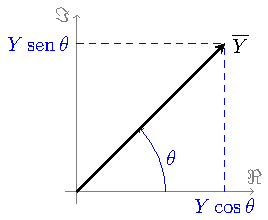
\includegraphics[height=0.45\textheight]{../figs/fasor.pdf}
\end{center}
\end{column}
\end{columns}
\end{frame}

\begin{frame}{Cálculo fasorial}
\begin{align*}
    \overline{Y_1}&=\overbrace{Y_{ef1}\,\cos(\theta_1)}^{a_1}+\mathrm{j}\,\overbrace{Y_{ef1}\,\sin(\theta_1)}^{b_1}=Y_{ef1}\phase{\theta_1}\\
    \overline{Y_2}&=\underbrace{Y_{ef2}\,\cos(\theta_2)}_{a_2}+\mathrm{j}\,\underbrace{Y_{ef2}\,\sin(\theta_2)}_{b_2}=Y_{ef2}\phase{\theta_2}
\end{align*}
    \begin{itemize}
        \item Forma binómica:
        \begin{itemize}
            \item Suma: $\overline{Y_1}+\overline{Y_2}=(a_1+a_2)+\mathrm{j}\,(b_1+b_2)$
            \item Resta: $\overline{Y_1}-\overline{Y_2}=(a_1-a_2)+\mathrm{j}\,(b_1-b_2)$
        \end{itemize}
        \item Forma polar:
        \begin{itemize}
            \item Multiplicar: $\overline{Y_1}\cdot \overline{Y_2}=(Y_{ef1}\cdot Y_{ef2})\phase{\theta_1+\theta_2}$
            \item Dividir: $\dfrac{\overline{Y_1}}{\overline{Y_2}}=\dfrac{Y_{ef1}}{Y_{ef2}}\phase{\theta_1-\theta_2}$
        \end{itemize}
    \end{itemize}
\end{frame}

\subsection{Representación fasorial: diagramas fasoriales}

\begin{frame}{Representación fasorial: diagramas fasoriales}{Tensión y corriente en notación fasorial} 
\begin{center}
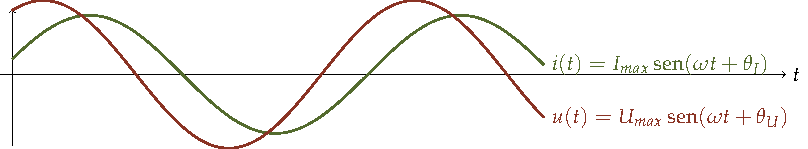
\includegraphics[width=.9\linewidth]{../figs/ondasTensionCorriente.pdf}
\end{center}

\begin{columns}
\begin{column}{0.5\columnwidth}
\begin{align*}
  \overline{U} &= U\phase{\theta_U}\\
  \overline{I} &= I\phase{\theta_I}
\end{align*}
\begin{block}{Importancia}
 \begin{itemize}
     \item Estudio y análisis de CA con vectores
     \item Relaciones claras e intuitivas
 \end{itemize}
\end{block}
\end{column}

\begin{column}{0.5\columnwidth}
\begin{center}
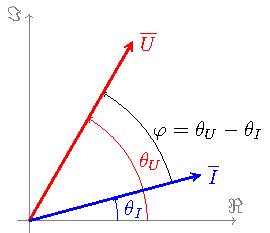
\includegraphics[height=0.5\textheight]{../figs/fasorTensionCorriente.pdf}
\end{center}
\end{column}
\end{columns}
\end{frame}

\section{Respuesta de los elementos pasivos a una excitación senoidal}

\subsection{Impedancia operacional}

\begin{frame}{Impedancia operacional}
{Relación entre fasores de tensión y corriente}
\begin{columns}
\begin{column}{0.5\columnwidth}
\begin{align*}
  \overline{U} &= \overline{Z} \cdot \overline{I}\\                 
  \overline{Z} &= \frac{\overline{U}}{\overline{I}}
\end{align*}

\[
\boxed{\overline{Z} = \frac{U}{I}\phase{\theta_U - \theta_I} \Rightarrow 
    \begin{cases}
      Z = \frac{U}{I}\\
      \theta = \theta_U - \theta_I
    \end{cases}}
\]
\end{column}


\begin{column}{0.5\columnwidth}
\begin{center}
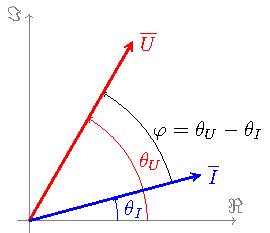
\includegraphics[height=0.5\textheight]{../figs/fasorTensionCorriente.pdf}
\end{center}
\end{column}
\end{columns}

% \begin{block}{Convenio de origen de fases}
%  \[
% \theta_U=0 \Rightarrow \begin{cases}
%       Z = \frac{U}{I}\\
%       \theta = -\theta_I
%      \end{cases}
%  \]
% \end{block}
\end{frame}

\begin{frame}{Impedancia operacional}
\[
\overline{Z}=Z\cdot\cos(\theta)+\mathrm{j}\,Z\cdot\sin(\theta) = R + \mathrm{j} X
\]

\begin{center}
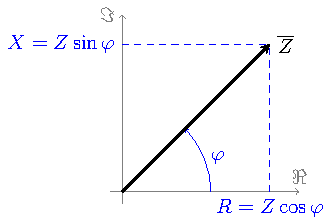
\includegraphics[height=0.75\textheight]{../figs/fasorImpedancia.pdf}
\end{center}
\end{frame}

\subsection{Circuito resistivo}

\begin{frame}{Circuito resistivo}
Un circuito resistivo no desfasa (\alert{tensión y corriente en fase})

\[
    i(t) = I\,\sqrt{2} \cdot \sin(\omega t + \theta_I)
\]
\[
  u(t) = R \cdot i(t)= {\color{blue}R\cdot I\,\sqrt{2}} \cdot \sin(\omega t + {\color{red!80}\theta_I}) = {\color{blue}U\,\sqrt{2}} \cdot \sin(\omega t + {\color{red!80} \theta_I})
\]

\begin{center}
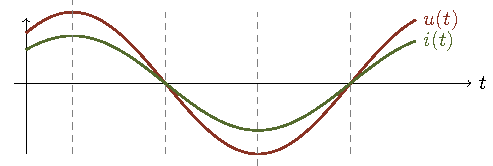
\includegraphics[height=0.4\textheight]{../figs/resistivo.pdf}
\end{center}
\end{frame}

\begin{frame}{Circuito resistivo}
Un circuito resistivo no desfasa (\alert{tensión y corriente en fase}).
\begin{center}
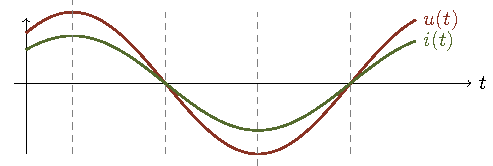
\includegraphics[height=0.3\textheight]{../figs/resistivo.pdf}
\end{center}

\begin{columns}
\begin{column}{0.3\columnwidth}
\begin{align*}
  Z &= \frac{U}{I} = R\\
  \theta &= \theta_U - \theta_I = 0\\
  \Aboxed{\overline{Z}_R &= R \phase{0}}
\end{align*}
\end{column}

\begin{column}{0.35\columnwidth}
\begin{center}
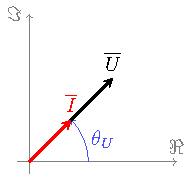
\includegraphics[height=0.35\textheight]{../figs/fasorResistencia_VI.pdf}
\end{center}
\end{column}


\begin{column}{0.35\columnwidth}
\begin{center}
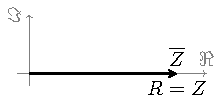
\includegraphics[height=0.25\textheight]{../figs/fasorResistencia.pdf}
\end{center}
\end{column}
\end{columns}
\end{frame}

\subsection{Circuito inductivo puro}

\begin{frame}{Circuito inductivo puro}
Un circuito inductivo puro genera \alert{señales en cuadratura} y \alert{retrasa la corriente}

\[
    i(t) = I\,\sqrt{2} \cdot \sin(\omega t + \theta_I)
\]
\[
  u(t) = L \cdot \frac{d i(t)}{dt} =
       {\color{blue}{\omega L I\,\sqrt{2}}} \cdot \underbrace{\cos(\omega t+{\color{red}\theta_I})}_{\sin(\omega t+{\color{red}{\theta_I}+\pi/2})} = {\color{blue}{U\,\sqrt{2}}} \cdot \sin(\omega t +  {\color{red!80}{\theta_I +\pi/2}})
\]

\begin{center}
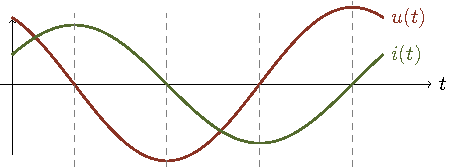
\includegraphics[height=0.3\textheight]{../figs/inductivoPuro.pdf}
\end{center}
\end{frame}

\begin{frame}{Circuito inductivo puro}
Un circuito inductivo puro genera \alert{señales en cuadratura} y \alert{retrasa la corriente}

\begin{center}
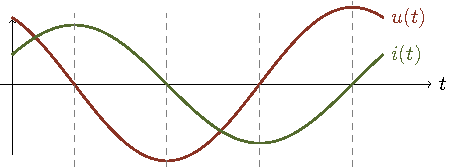
\includegraphics[height=0.3\textheight]{../figs/inductivoPuro.pdf}
\end{center}

\begin{columns}
\begin{column}{0.3\columnwidth}
\begin{align*}
  Z &= \frac{U}{I} = \omega L\\
  \theta &= \theta_U - \theta_I = \pi/2\\
  \Aboxed{\overline{Z}_L &= \mathrm{j}\omega L = \omega L \phase{\ang{90}}}
\end{align*}
\end{column}


\begin{column}{0.4\columnwidth}
\begin{center}
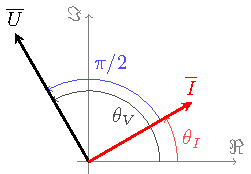
\includegraphics[height=0.4\textheight]{../figs/fasorInductancia_VI.pdf}
\end{center}
\end{column}


\begin{column}{0.3\columnwidth}
\begin{center}
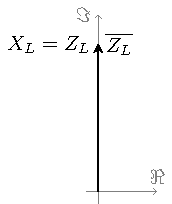
\includegraphics[height=0.4\textheight]{../figs/fasorInductancia.pdf}
\end{center}
\end{column}
\end{columns}
\end{frame}

\subsection{Circuito capacitivo puro}

\begin{frame}{Circuito capacitivo puro}
Un circuito capacitivo puro genera \alert{señales en cuadratura} y \alert{adelanta la corriente}

\[
    i(t) = I\,\sqrt{2} \cdot \sin(\omega t + \theta_I)
\]
\[
 u(t)=\dfrac{1}{C}\cdot\int_{-\infty}^{t} i(t)\cdot dt={\color{blue}\dfrac{I}{\omega\,C}\sqrt{2}}\cdot\underbrace{(-\cos (\omega t+{\color{red}\theta_I}))}_{\sin(\omega t+{\color{red}\theta_I-\pi/2})}={\color{blue}U\sqrt{2}}\cdot\sin \left(\omega t+{\color{red}\theta_I-\pi/2}\right)
\]
     

\begin{center}
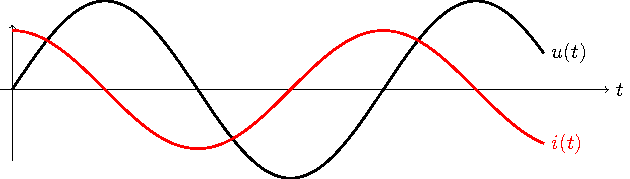
\includegraphics[height=0.3\textheight]{../figs/capacitivoPuro.pdf}
\end{center}
\end{frame}


\begin{frame}{Circuito capacitivo puro}
Un circuito capacitivo puro genera \alert{señales en cuadratura} y \alert{adelanta la corriente}

\begin{center}
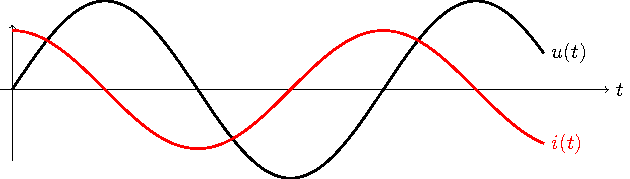
\includegraphics[height=0.3\textheight]{../figs/capacitivoPuro.pdf}
\end{center}

\begin{columns}
\begin{column}{0.3\columnwidth}
\begin{align*}
  Z &= \frac{U}{I} = \frac{1}{\omega C}\\
  \theta &= \theta_U - \theta_I = - \pi/2\\
  \Aboxed{\overline{Z}_C &= \frac{1}{\mathrm{j}\omega C} = \frac{1}{\omega C}\phase{\ang{-90}}}
\end{align*}
\end{column}


\begin{column}{0.4\columnwidth}
\begin{center}
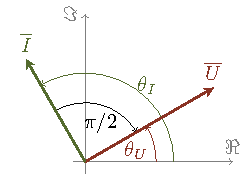
\includegraphics[height=0.4\textheight]{../figs/fasorCondensador_VI.pdf}
\end{center}
\end{column}


\begin{column}{0.3\columnwidth}
\begin{center}
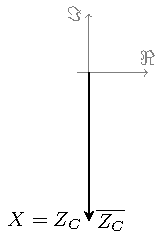
\includegraphics[height=0.4\textheight]{../figs/fasorCondensador.pdf}
\end{center}
\end{column}
\end{columns}
\end{frame}

\section{Respuesta de los circuitos serie a una excitación senoidal}

\subsection{Circuito RL}

\begin{frame}{Circuito RL}
\begin{center}
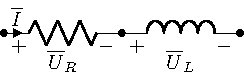
\includegraphics[height=0.2\textheight]{../figs/RL.pdf}
\end{center}

\begin{columns}
\begin{column}{0.45\columnwidth}
\begin{align*}
&\overline{I}=I\phase{\theta_I}\\
    &\overline{U_R} = R \overline{I}=R\cdot I\phase{\theta_I}\\ 
	&\overline{U_L}=\overline{X_L}\cdot\overline{I}= \omega\,L\,I\phase{\theta_I+90^\circ}
\end{align*}
\end{column}

\begin{column}{0.55\columnwidth}
\begin{equation*}
  \overline{U} = \overline{U}_R + \overline{U}_L =(\underbrace{R + \mathrm{j}\,\omega L}_{\overline{Z_{eq}}})\; \overline{I}
\end{equation*}
\end{column}
\end{columns}
\end{frame}

\begin{frame}{Circuito RL}
\begin{center}
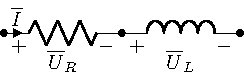
\includegraphics[height=0.2\textheight]{../figs/RL.pdf}
\end{center}

\begin{columns}
\begin{column}{0.45\columnwidth}
\[
\overline{Z} = R + \mathrm{j}\omega L \Rightarrow \boxed{\theta > 0}
\]
\begin{align*}
    Z &= \sqrt{R^2 + (\omega L)^2}\\
    \theta &= \arctan{\frac{\omega L}{R}}
\end{align*}
\end{column}

\begin{column}{0.55\columnwidth}
\begin{center}
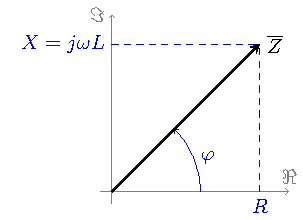
\includegraphics[width=.9\linewidth]{../figs/fasorInductanciaReal.pdf}
\end{center}
\end{column}
\end{columns}
\end{frame}

\begin{frame}{Circuito RL}
\begin{columns}
\begin{column}{0.7\columnwidth}
\begin{center}
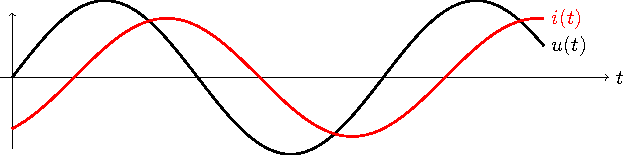
\includegraphics[width=\linewidth]{../figs/inductivo.pdf}
\end{center}
\end{column}
\begin{column}{0.25\columnwidth}
\begin{center}
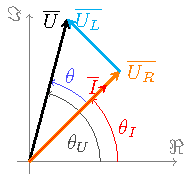
\includegraphics[width=\linewidth]{../figs/fasorInductanciaReal_VI.pdf}
\end{center}
\end{column}
\end{columns}

\begin{center}
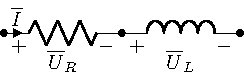
\includegraphics[height=0.15\textheight]{../figs/RL.pdf}
\begin{equation*}
		\overline{U} = \overline{U_R} + \overline{U_L} =(R + \mathrm{j}\,\omega L) \cdot \overline{I}\Rightarrow 
		\begin{cases}
			U=\sqrt{U_R^2+U_L^2}=I\sqrt{R^2+(\omega L)^2}=I\cdot Z_{eq}\\
			\theta=\arctan\left( \dfrac{U_L}{U_R}\right)=\arctan\left( \dfrac{\omega L}{R}\right)
		\end{cases}
	\end{equation*}
\end{center}
\end{frame}

\subsection{Circuito RC} 

\begin{frame}{Circuito RC}
\begin{center}
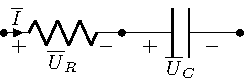
\includegraphics[height=0.2\textheight]{../figs/RC.pdf}
\end{center}

\begin{columns}
\begin{column}{0.45\columnwidth}
\begin{align*}
&\overline{I}=I\phase{\theta_I}\\
    &\overline{U_R} = R \overline{I}=R\cdot I\phase{\theta_I}\\ 
	&\overline{U_C}=\overline{X_C}\cdot\overline{I}= \dfrac{I}{\omega\,C}\,I\phase{\theta_I-90^\circ}
\end{align*}
\end{column}

\begin{column}{0.55\columnwidth}
\begin{equation*}
  \overline{U} = \overline{U}_R + \overline{U}_C =\underbrace{\left(R - \mathrm{j}\,\dfrac{1}{\omega C}\right)}_{\overline{Z_{eq}}}\; \overline{I}
\end{equation*}
\end{column}
\end{columns}
\end{frame}

\begin{frame}{Circuito RC}
\begin{center}
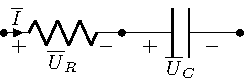
\includegraphics[height=0.2\textheight]{../figs/RC.pdf}
\end{center}

\begin{columns}
\begin{column}{0.45\columnwidth}
\[
\overline{Z} = R - \mathrm{j}\dfrac{1}{\omega C} \Rightarrow \boxed{\theta < 0}
\]
\begin{align*}
    Z &= \sqrt{R^2 - \left(\dfrac{1}{\omega C}\right)^2}\\
    \theta &= -\arctan{\frac{1}{R\,\omega\,C}}
\end{align*}
\end{column}

\begin{column}{0.55\columnwidth}
\begin{center}
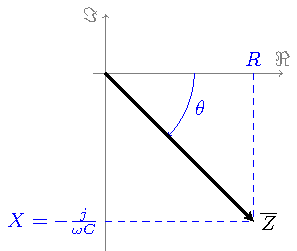
\includegraphics[width=.8\linewidth]{../figs/fasorCondensadorReal.pdf}
\end{center}
\end{column}
\end{columns}
\end{frame}

\begin{frame}{Circuito RC}
\begin{columns}
\begin{column}{0.7\columnwidth}
\begin{center}
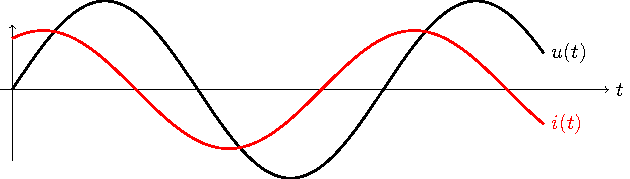
\includegraphics[width=\linewidth]{../figs/capacitivo.pdf}
\end{center}
\end{column}
\begin{column}{0.25\columnwidth}
\begin{center}
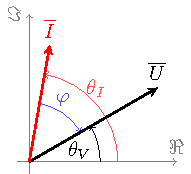
\includegraphics[width=\linewidth]{../figs/fasorCondensadorReal_VI.pdf}
\end{center}
\end{column}
\end{columns}

\begin{center}
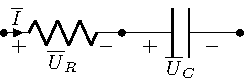
\includegraphics[height=0.15\textheight]{../figs/RC.pdf}
\begin{equation*}
		\overline{U} = \overline{U_R} + \overline{U_C} =\left(R - \mathrm{j}\,\dfrac{1}{\omega\,C}\right) \cdot \overline{I}\Rightarrow 
		\begin{cases}
			U=\sqrt{U_R^2+U_C^2}=I\sqrt{R^2+\left(\dfrac{1}{\omega\,C}\right)^2}=I\cdot Z\\
			\theta=-\arctan\left( \dfrac{U_C}{U_R}\right)=-\arctan\left( \dfrac{1}{R\,\omega\,C}\right)
		\end{cases}
	\end{equation*}
\end{center}
\end{frame}

\subsection{Circuito RLC}

\begin{frame}{Circuito RLC}
\begin{center}
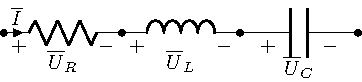
\includegraphics[height=0.2\textheight]{../figs/RLC.pdf}
\end{center}

\begin{columns}
\begin{column}{0.45\columnwidth}
\begin{align*}
&\overline{I}=I\phase{\theta_I}\\
    &\overline{U_R} = R \overline{I}=R\cdot I\phase{\theta_I}\\ 
    &\overline{U_L}=\overline{X_L}\cdot\overline{I}= \omega\,L\,I\phase{\theta_I+90^\circ}\\
	&\overline{U_C}=\overline{X_C}\cdot\overline{I}= \dfrac{I}{\omega\,C}\,I\phase{\theta_I-90^\circ}
\end{align*}
\end{column}

\begin{column}{0.55\columnwidth}
\begin{equation*}
  \overline{U} = \overline{U}_R + \overline{U}_L + \overline{U}_C =\underbrace{\left(R + \mathrm{j}\,\omega\,L - \mathrm{j}\,\dfrac{1}{\omega C}\right)}_{\overline{Z_{eq}}}\; \overline{I}
\end{equation*}
\end{column}
\end{columns}
\end{frame}

\begin{frame}{Circuito RLC}
\begin{center}
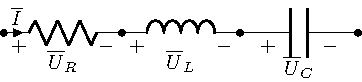
\includegraphics[height=0.2\textheight]{../figs/RLC.pdf}
\end{center}

\begin{columns}
\begin{column}{0.45\columnwidth}
\[
\overline{Z} = R+ \mathrm{j}\left(\omega\,L-\dfrac{1}{\omega C}\right) \Rightarrow \boxed{\theta?}
\]
\begin{align*}
    Z &= \sqrt{R^2+\left(\omega L -\frac{1}{\omega C} \right)^2}\\
    \theta&=\arctan\left(\dfrac{\omega L-\frac{1}{\omega\,C}}{R} \right)
\end{align*}
\end{column}

\begin{column}{0.55\columnwidth}
\begin{itemize}
\item \(\theta > 0 \Rightarrow \omega L > \frac{1}{\omega C}\): inductivo
\item \(\theta < 0 \Rightarrow \omega L < \frac{1}{\omega C}\): capacitivo
\item \(\theta = 0 \Rightarrow \omega L = \frac{1}{\omega C}\): resistivo (resonancia)
\end{itemize}
\end{column}
\end{columns}
\end{frame}

\begin{frame}{Circuito RLC}
\begin{columns}
\begin{column}{0.5\columnwidth}
\begin{center}
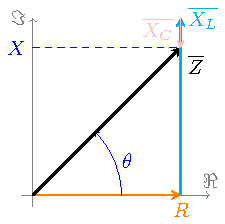
\includegraphics[width=0.6\linewidth]{../figs/fasorRLC.pdf}
\end{center}
\end{column}
\begin{column}{0.5\columnwidth}
\begin{center}
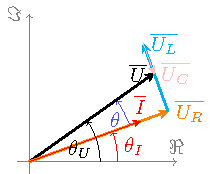
\includegraphics[width=0.6\linewidth]{../figs/fasorRLC_VI.pdf}
\end{center}
\end{column}
\end{columns}

\begin{center}
\begin{equation*}
		\overline{U} = \overline{U_R} +\overline{U_L} + \overline{U_C} =\left(R+\mathrm{j}\,\omega\,L - \mathrm{j}\,\dfrac{1}{\omega\,C}\right) \cdot \overline{I}\Rightarrow 
		\begin{cases}
			U=I\sqrt{R^2 + \left(\omega L - \dfrac{1}{\omega C}\right)^2}=I\cdot Z\\
			\theta=\arctan\left( \dfrac{\omega\,L-\frac{1}{\omega\,C}}{R}\right)
		\end{cases}
	\end{equation*}
\end{center}
\end{frame}

\subsection{Circuito serie general}

\begin{frame}{Circuito serie general}
\begin{columns}
\begin{column}{0.7\linewidth}
\begin{center}
    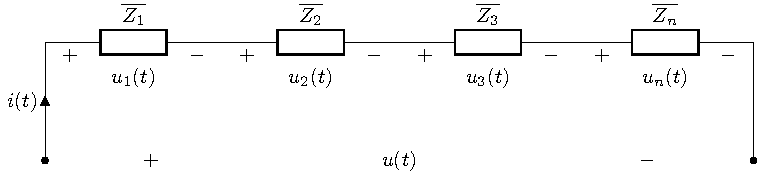
\includegraphics[height=2cm]{../figs/serie_general.pdf}
\end{center}
\end{column}
\begin{column}{0.3\linewidth}
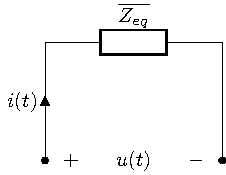
\includegraphics[height=2cm]{../figs/serie_general_eq.pdf}
\end{column}
\end{columns}

\begin{equation*}
		\overline{U}=\overline{U_1}+\overline{U_2}+\overline{U_3}+...+\overline{U_n}=\overline{I} \cdot(\overline{Z_1}+\overline{Z_2}+\overline{Z_3}+...+\overline{Z_n})=\overline{I}\cdot\overline{Z_{eq}}
	\end{equation*}
	\begin{equation*}
		\overline{Z_{eq}}=\overline{Z_1}+\overline{Z_2}+\overline{Z_3}+...+\overline{Z_n}\Rightarrow \boxed{\overline{Z_{eq}}=\sum_{i=1}^n \overline{Z_i}}
	\end{equation*}
	\begin{equation*}
		R_{eq}=\sum_{i=1}^n R_i\,;\qquad \qquad X_{eq}=\sum_{i=1}^n X_i
	\end{equation*}
	\begin{equation*}
		\theta=\arctan\left(\dfrac{X_{eq}}{R_{eq}}\right)
	\end{equation*}
\end{frame}

\begin{frame}{Circuito serie general}{Ejemplo}
    Un circuito en serie formado por $R=\si{10}{\ohm}$, $L=\qty{20}{\milli\henry}$ y $C=\qty{100}{\micro\farad}$ se conecta a una tensión $u(t)=\qty[parse-numbers = false]{200\cdot\sin(1000t+\frac{\pi}{4})}{\volt}$. Calcular $\overline{I}$, ${u_R(t)}$, $u_L(t)$ y $u_C(t)$ y dibujar el diagrama fasorial
\end{frame}

\section{Respuesta de los circuitos paralelo a una excitación senoidal}

\begin{frame}{Circuito paralelo general}
\begin{columns}
\begin{column}{0.7\linewidth}
\begin{center}
    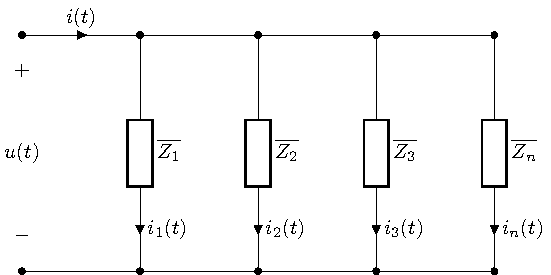
\includegraphics[height=3cm]{../figs/paralelo_general.pdf}
\end{center}
\end{column}
\begin{column}{0.3\linewidth}
\begin{center}
    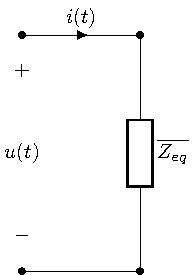
\includegraphics[height=3cm]{../figs/paralelo_general_eq.pdf}
\end{center}
\end{column}
\end{columns}

\begin{equation*}
		\overline{I}=\overline{I_1}+\overline{I_2}+\overline{I_3}+...+\overline{I_n}=\overline{U} \cdot\left(\dfrac{1}{\overline{Z_1}}+\dfrac{1}{\overline{Z_2}}+\dfrac{1}{\overline{Z_3}}+...+\dfrac{1}{\overline{Z_n}}\right)=\dfrac{\overline{U}}{\overline{Z_{eq}}}
	\end{equation*}
	\begin{equation*}
		\dfrac{1}{\overline{Z_{eq}}}=\dfrac{1}{\overline{Z_1}}+\dfrac{1}{\overline{Z_2}}+\dfrac{1}{\overline{Z_3}}+...+\dfrac{1}{\overline{Z_n}}\Rightarrow \boxed{\dfrac{1}{\overline{Z_{eq}}}=\dfrac{1}{\displaystyle\sum_{i=1}^n \overline{Z_i}}}
	\end{equation*}
\end{frame}

\subsection{Admitancia}

\begin{frame}{Impedancia y admitancia}
\begin{columns}
\begin{column}{0.5\columnwidth}
\begin{center}
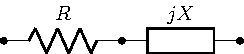
\includegraphics[height=0.1\textheight]{../figs/Z.pdf}
\end{center}
\[
  \overline{U} = \overline{Z} \cdot \overline{I}
\]
\[
  \overline{Z} = R + \mathrm{j} X
\]
\end{column}

\begin{column}{0.5\columnwidth}
\begin{center}
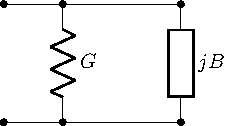
\includegraphics[height=0.25\textheight]{../figs/Y.pdf}
\end{center}
\[
  \overline{I} = \overline{Y} \cdot \overline{U}
\]
\[
  \overline{Y} = G + \mathrm{j} B
\]
\end{column}
\end{columns}

\[
\boxed{
  \overline{Y} = \frac{1}{\overline{Z}} \rightarrow \left\{%
    \begin{array}{l}
      |Y| = \frac{1}{|Z|}\\
      \theta_Y = -\theta_Z = -\theta\\
      \end{array}\right.
      }
\]
\end{frame}

\begin{frame}{Impedancia y admitancia}
\begin{columns}
\begin{column}{0.5\columnwidth}
\begin{center}
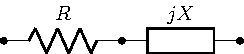
\includegraphics[height=0.1\textheight]{../figs/Z.pdf}
\end{center}

\[
  \overline{Z} = \frac{1}{G + \mathrm{j} B} \rightarrow \left\{%
      \begin{array}{l}
	R = \dfrac{G}{G^2 + B^2}\\[5mm]
	X = - \mathrm{j} \dfrac{B}{G^2 + B^2}\\
      \end{array}\right.        
\]
\end{column}

\begin{column}{0.5\columnwidth}
\begin{center}
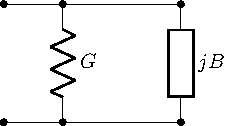
\includegraphics[height=0.25\textheight]{../figs/Y.pdf}
\end{center}

\[
  \overline{Y} = \frac{1}{R + \mathrm{j} X} \rightarrow \left\{%
      \begin{array}{l}
	G = \dfrac{R}{R^2 + X^2}\\[5mm]
	B = - \mathrm{j} \dfrac{X}{R^2 + X^2}\\
      \end{array}\right.        
\]
\end{column}
\end{columns}
\end{frame}

\begin{frame}{Impedancia y admitancia}{Ejemplo}
    Calcular la impedancia y admitancia compleja equivalente del circuito de la figura.
	    \begin{figure}[H]
	        \centering
	        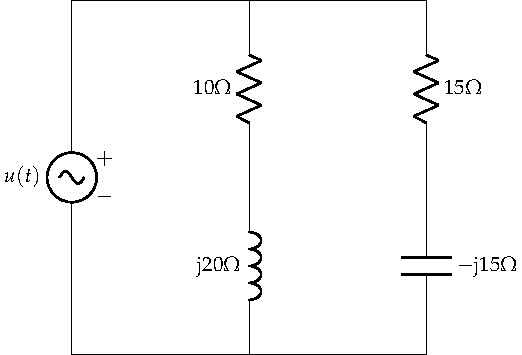
\includegraphics{../figs/impedancia_admitancia_eq.pdf}
	    \end{figure}
\end{frame}



\section{Potencia en corriente alterna}
\begin{frame}{Potencia en corriente alterna}{Potencia instantánea}
Sea la tensión referencia de fases. Si \(\theta > 0\) (inductivo) la corriente está retrasada respecto de la tensión (\emph{circuito en retraso}).
\begin{align*}
  u(t) &= U\sqrt{2} \cos (\omega t)\\
  i(t) &= I\sqrt{2} \cos (\omega t {\color{red}-} \theta)\\
  p(t) &= u(t) \cdot i(t)
\end{align*}

\begin{equation*}
  p(t)=\left(U\sqrt{2}\cdot \cos (\omega t) \right)\cdot \left(I\sqrt{2} \cdot \cos (\omega t -\theta)\right)=2\cdot U\cdot I\cdot \cos(\omega t)\cdot\cos(\omega t-\theta)
\end{equation*}

\begin{equation*}
		p(t)=2\cdot U\cdot I\cdot \overbrace{\cos(\omega t)}^{\cos(\alpha)}\cdot\overbrace{\cos(\omega t-\theta)}^{\cos(\beta)}\Rightarrow \boxed{p(t)
			=U\cdot I \cdot \cos(\theta)+U\cdot I \cdot\cos(2\omega t-\theta)}
	\end{equation*}
\end{frame}

\begin{frame}{Potencia en corriente alterna}{Potencia instantánea} 
$p(t)$ cambia con el tiempo. El valor medio en un periodo:
	\begin{equation*}
		P_m=\dfrac{1}{T}\int_{0}^{T}p(t)\,dt=\dfrac{1}{T}\int_{0}^{T}U\,I\,\cos(\theta)\,dt+\cancelto{0}{\dfrac{1}{T}\int_{0}^{T}U\,I\,\cos(2\omega t-\theta)\,dt}=U\,I\,\cos(\theta)
	\end{equation*}
	que coincide con el \alert{término fijo} de $p(t)$ y se conoce como \alert{potencia activa}. El término $U\,I\,\cos(2\omega t-\theta)$ es el responsable de que $p(t)$ fluctúe en torno a $P$, conociéndose como \alert{potencia fluctuante}. Teniendo en cuenta la relación para el coseno de una resta: 
	\begin{equation*}
		p(t)=\underbrace{{\color{blue}U\,I\,\cos(\theta)}\left[1+\cos(2\omega t)\right]}_{p_1(t)} + \underbrace{{\color{red}U\,I\sin(\theta)}\,\sin(2\omega t)}_{p_2(t)}={\color{blue}P}\left[1+\cos(2\omega t)\right] + {\color{red}Q}\,\sin(2\omega t)
	\end{equation*}
	\end{frame}
	
	\begin{frame}{Potencia en corriente alterna}{Expresión general}
	\begin{itemize}
		\item $P$, positiva, es la potencia media que consumen los elementos resistivos, y se denomina \alert{potencia activa} [W]:
		\begin{equation*}
			\boxed{P=U\,I\,\cos(\theta)}
		\end{equation*}
		\item $Q$, positiva o negativa, es la máxima potencia que almacena/devuelve el circuito (no implica transformación en trabajo útil), y se denomina \alert{potencia reactiva} [VAr]:
		\begin{equation*}
			\boxed{Q=U\,I\,\sin(\theta)}
		\end{equation*}
	\end{itemize}
\end{frame}

\subsection{Circuito resistivo}

\begin{frame}{Circuito resistivo}
   \[
     P = UI\cos(\theta) \qquad%
     {\color{gray}Q = UI\sin(\theta)}
   \]
   
   \begin{equation*}
p(t) = P\,\left[1+\cos(2\omega t)\right] + {\color{gray}Q\,\sin(2\omega t)}
\end{equation*}

\noindent\rule{\textwidth}{0.5pt}
\[
  \overline{Z_R}=R\phase{0^\circ}\rightarrow\theta = 0 \rightarrow%
  \left\{% 
    \begin{array}{l}
      P = UI = \dfrac{U^2}{R} = I^2 R\\
      Q = 0\\
    \end{array}
    \right.
  \]

  \[
    p(t) = P \cdot (1 + \cos(2 \omega t))
  \]
\end{frame}

\begin{frame}{Circuito resistivo}
\begin{center}
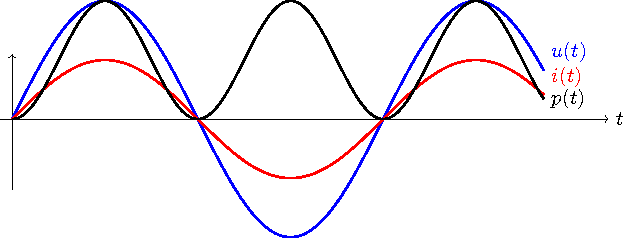
\includegraphics[width=.9\linewidth]{../figs/resistivoPotencia.pdf}
\end{center}

\begin{itemize}
\item Fluctúa al doble de frecuencia
\item Es siempre positiva
\end{itemize}
\end{frame}

\subsection{Circuito inductivo puro}

\begin{frame}{Circuito inductivo puro}
   \[
     {\color{gray}P = UI\cos(\theta)} \qquad%
     Q = UI\sin(\theta)
   \]
   
   \begin{equation*}
p(t) = {\color{gray}P \left[1 + \cos(2\omega t)\right]} + Q \cdot \sin(2\omega t)
\end{equation*}

\noindent\rule{\textwidth}{0.5pt}

\[
 \overline{Z_L}=\omega\,L\phase{90^\circ}\rightarrow \theta = 90 \rightarrow%
  \left\{% 
    \begin{array}{l}
      P = 0\\
      Q = UI = \dfrac{U^2}{\omega L} = I^2 \omega L\\
    \end{array}
    \right.
  \]

\[
  p(t) = Q \cdot \sin(2 \omega t)
\]
\end{frame}

\begin{frame}{Circuito inductivo puro}
\begin{center}
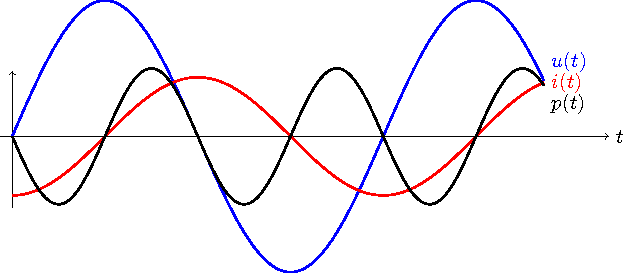
\includegraphics[width=.9\linewidth]{../figs/inductivoPuroPotencia.pdf}
\end{center}

\begin{itemize}
\item Fluctúa al doble de frecuencia
\item Pasa por los ceros de tensión y corriente
\item Su valor medio es nulo
\end{itemize}
\end{frame}

\begin{frame}{Circuito capacitivo puro}
   \[
     {\color{gray}P = UI\cos\theta} \qquad%
     Q = UI\sin\theta
   \]
   
   \begin{equation*}
p(t) = {\color{gray}P \left[1 + \cos(2\omega t)\right]} + Q \cdot \sin(2\omega t)
\end{equation*}

\noindent\rule{\textwidth}{0.5pt}

\[
  \overline{Z_C}=\dfrac{1}{\omega\,C}\phase{-90^\circ}\rightarrow\theta = -90 \rightarrow%
  \left\{% 
    \begin{array}{l}
      P = 0\\
      Q = -UI = -U^2 \omega C = - \dfrac{I^2}{\omega C}\\
    \end{array}
    \right.
  \]
\[
  p(t) = Q \cdot \sin(2 \omega t)
\]
\end{frame}

\begin{frame}{Circuito capacitivo puro}
\begin{center}
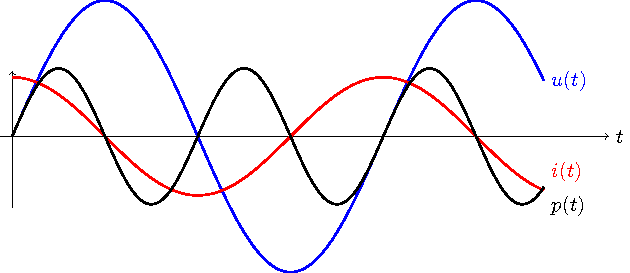
\includegraphics[width=.9\linewidth]{../figs/capacitivoPuroPotencia.pdf}
\end{center}

\begin{itemize}
\item Fluctúa al doble de frecuencia
\item Pasa por los ceros de tensión y corriente
\item Su valor medio es nulo
\end{itemize}
\end{frame}

% \begin{frame}[label={sec:orgedf0da0}]{Circuito Inductivo con pérdidas}
% \begin{center}
% 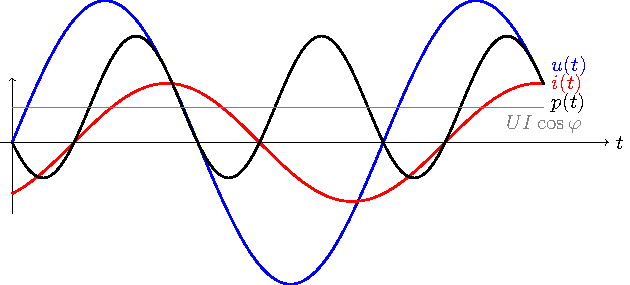
\includegraphics[height=0.5\textheight]{../figs/inductivoPotencia.pdf}
% \end{center}

% \[
%      p(t) = P \cdot (1 + \cos(2\omega t)) + Q \cdot \sin(2\omega t)
% \]

% \begin{center}
% Valor medio positivo, \(P = U I \cos \theta\)
% \end{center}
% \end{frame}


% \begin{frame}[label={sec:org1ffbf27}]{Circuito Capacitivo con pérdidas}
% \begin{center}
% 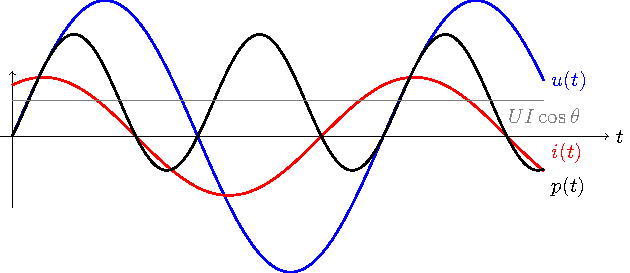
\includegraphics[height=0.5\textheight]{../figs/capacitivoPotencia.pdf}
% \end{center}

% \[
%      p(t) = P \cdot (1 + \cos(2\omega t)) + Q \cdot \sin(2\omega t)
% \]

% \begin{center}
% Valor medio positivo, \(P = U I \cos \theta\)
% \end{center}
% \end{frame}

\subsection{Triángulo de potencias}

\begin{frame}{Triángulo de potencias}
\begin{columns}
\begin{column}{0.6\columnwidth}
\begin{itemize}
\item Potencia activa [W]
\end{itemize}
\[  
\boxed{P = U\cdot I\cdot\cos(\theta) = R \cdot I^2}
\]

\begin{itemize}
\item Potencia reactiva [VAr]
\end{itemize}
\[
\boxed{Q = U\cdot I\cdot\sin(\theta) = X \cdot I^2}
\]

\begin{itemize}
\item Potencia aparente [VA]
\end{itemize}
\[
\boxed{\overline{S} = P + \mathrm{j}Q = \overline{U} \cdot \overline{I}^*}
\]
{\begin{align*}
  \overline{U} &= U\phase{0}\\
  \overline{I} &= I\phase{-\theta}\\
\overline{U}\;\overline{I}^* &= U\phase{0} \cdot I\phase{\theta} = UI\phase{\theta}=\\
&=U I (\cos\theta + \mathrm{j} \sin\theta) = P + \mathrm{j} Q
\end{align*}}
\end{column}

\begin{column}{0.4\columnwidth}
\vspace{-10mm}
\begin{center}
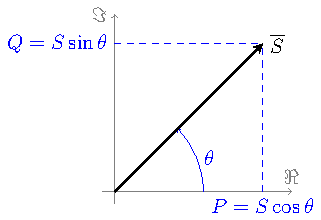
\includegraphics[width=.8\linewidth]{../figs/trianguloPotencias.pdf}
\end{center}

\[
S = U \cdot I
\]
\[
\theta_S = \theta_Z = \theta
\]
\[
f.d.p. \equiv \cos(\theta)
\]
\end{column}
\end{columns}
\end{frame}

\subsection{Resumen de potencia de los elementos pasivos}

\begin{frame}{Resumen de potencia de los elementos pasivos}{Resistencia}
\[
\theta = 0 \Rightarrow 
\begin{cases}
  P_R = R I^2\\
  Q_R = 0\\
  S_R = P_R
\end{cases}
\]

\begin{itemize}
\item Consume potencia activa
\item No consume potencia reactiva
\end{itemize}
\end{frame}

\begin{frame}{Resumen de potencia de los elementos pasivos}{Bobina}
\[
\theta = 90 \Rightarrow 
\begin{cases}
  P_L = 0\\
  Q_L = \omega L I^2\\
  \overline{S}_L = \omega L I^2 \phase{90^\circ}
\end{cases}
\]

\begin{itemize}
\item No consume potencia activa
\item Consume potencia reactiva (\(Q > 0\))
\end{itemize}
\end{frame}

\begin{frame}{Resumen de potencia de los elementos pasivos}{Condensador}

\[
\theta = - 90 \Rightarrow 
\begin{cases}
  P_L = 0\\
  Q_C = - \omega C U^2\\
  \overline{S}_C = \omega C U^2 \phase{-90^\circ}
\end{cases}
\]

\begin{itemize}
\item No consume potencia activa
\item Genera potencia reactiva (\(Q < 0\))
\end{itemize}
\end{frame}

\subsection{Teorema de Boucherot}

\begin{frame}{Teorema de Boucherot}
\begin{itemize}
\item Consecuencia del \alert{principio de conservación de la energía}
\item Supóngase $\overline{Z_1}=R_1+\mathrm{j}\,X_1$, $\overline{Z_2}=R_2+\mathrm{j}\,X_2$ y $\overline{Z_3}=R_3-\mathrm{j}\,X_3$ en serie recorridas por $\overline{I}=I\phase{0^\circ}$:
	\begin{equation*}
		\overline{U}=\sum_{i=1}^3 \overline{U_i}\Rightarrow
		\begin{cases}
			U\,\cos(\theta)=\displaystyle\sum_{i=1}^3 U_i\,\cos(\theta_i)\\
			U\,\sin(\theta)=\displaystyle\sum_{i=1}^3 U_i\,\sin(\theta_i)
		\end{cases}
	\end{equation*}
	Multiplicando las dos expresiones por ${I}$: 
	\begin{align*}
		U\,I\,\cos(\theta)&=P_T=\displaystyle\sum_{i=1}^3 U_i\,I\,\cos(\theta_i)=\displaystyle\sum_{i=1}^3 P_i\\
		U\,I\,\sin(\theta)&=Q_T=\displaystyle\sum_{i=1}^3 U_i\,I\,\sin(\theta_i)=\displaystyle\sum_{i=1}^3 Q_i
	\end{align*}
\end{itemize}
\end{frame}

\begin{frame}{Teorema de Boucherot}
La potencia aparente total es la suma de las potencias aparentes individuales (la potencia activa/reactiva total es la suma de las potencias activas/reactivas individuales):
\begin{columns}
\begin{column}{0.3\columnwidth}
\begin{align*}
  \overline{S} &= \sum_{i = 1}^{n} \overline{S}_i\\
  P_T + \mathrm{j}Q_T &= \sum^n_{i = 1} (P_i + \mathrm{j}Q_i)
\end{align*}
\end{column}
\begin{column}{0.7\linewidth}
\begin{figure}
		\centering
		\includegraphics[width=\linewidth]{../figs/boucherot.pdf}
	\end{figure}
\end{column}
\end{columns}
\end{frame}

\begin{frame}{Teorema de Boucherot}{Ejemplo}
    Sabiendo que las fuentes de tensión del circuito de la figura vienen definidas por las formas de onda $u_1(t)=10\sqrt{2}\cdot \cos(1000\cdot t)$ V y $u_2(t)=5\sqrt{2}\cdot \sin(1000\cdot t)$ V, calcular las potencias de cada elemento, así como el balance de potencias del circuito. 
		\begin{figure}[H]
			\centering
			\includegraphics[width=0.6\linewidth]{../figs/ej7_BT2.pdf}
		\end{figure}
\end{frame}

\subsection{Medida de potencia: vatímetro}

\begin{frame}{Medida de potencia: vatímetro}
\begin{center}
\includegraphics[height=0.5\textheight]{../figs/vatimetro_2.pdf}
\end{center}

\alert{Vatímetro}: equipo de medida de 4 terminales (1 par para tensión, 1 par para corriente):

\begin{equation*}
	    W=\overline{I_{1,2}}\,\circ\,\overline{U_{3,4}}=I_{1,2}\cdot U_{3,4}\cdot \widehat{(I_{1,2}, U_{3,4})}
	\end{equation*}
\end{frame}

% \begin{frame}{Medida de potencia}
% \begin{center}
% \includegraphics[height=0.5\textheight]{../figs/vatimetro_2.pdf}
% \end{center}


% Habitualmente se emplea con 3 terminales cortocircuitando terminales con *.
% \[
%   \boxed{W = |V| |I| \cos(\theta_V - \theta_I) = P_Z}
% \]
% \end{frame}

\subsection{Factor de potencia: importancia y mejora}

\begin{frame}{Factor de potencia: importancia y mejora}
El factor de potencia, \(\cos(\theta)\), representa la aportación de potencia activa dentro de la potencia aparente:
\[
\cos (\theta)=\dfrac{P}{S}
\]

Se dice que:
	\begin{itemize}
		\item $\cos(\theta)$ \alert{en retraso} cuando el circuito tiene carácter inductivo (la intensidad va retrasada respecto a la tensión)
		\item $\cos(\theta)$ \alert{en adelanto} cuando el circuito tiene carácter capacitivo (la intensidad va adelantada respecto a la tensión)
	\end{itemize}
	
	\end{frame}

\begin{frame}{Factor de potencia: importancia y mejora}
Sean dos sistemas con \alert{misma tensión y potencia activa}, y factores de potencia \(\cos \theta_2 < \cos \theta_1\) (\(Q_2 > Q_1\))
\begin{columns}
\begin{column}{0.4\linewidth}
\begin{center}
\includegraphics[width=\linewidth]{../figs/fasorescompensacionreactiva.pdf}
\end{center}
\end{column}
\begin{column}{0.6\linewidth}
\begin{itemize}
    \item El sistema 2 requiere \alert{mayor potencia aparente} (generador mayor) para alimentar la misma potencia activa:
\[
  \left(\frac{P}{\cos \theta_1} = S_1 \right) < \left( S_2 = \frac{P}{\cos \theta_2}\right) 
\]
\item El sistema 2 requiere \alert{mayor sección} de cable para transportar la misma potencia activa:
\[
  \left(\frac{P}{U \cos \theta_1} = I_1 \right) < \left( I_2 = \frac{P}{U \cos \theta_2}\right) 
\]
\end{itemize}
\end{column}
\end{columns}
\end{frame}

\begin{frame}{Factor de potencia: importancia y mejora}
\begin{itemize}
\item Comúnmente, el factor de potencia es \alert{inductivo} (máquinas eléctricas
industriales)
\item Es necesario mejorar \alert{localmente} el factor de potencia: ¿qué elemento pasivo genera $Q$?
\pause\begin{itemize}
    \item \alert{Condensadores}
\end{itemize}
\end{itemize}

Sea una carga de potencia activa \(P_z\), potencia reactiva \(Q_z\), factor de potencia \(\cos\theta\). Se desea \alert{mejorar el factor de potencia} a \(\cos \theta' > \cos \theta\), manteniendo la potencia $P_z$
\end{frame}

\begin{frame}{Factor de potencia: importancia y mejora}
\begin{columns}
\begin{column}{0.4\linewidth}
\begin{center}
\includegraphics[width=\linewidth]{../figs/circuitocompensacionreactiva.pdf}
\end{center}
\begin{center}
\includegraphics[width=0.65\linewidth]{../figs/trianguloCompensacionQ.pdf}
\end{center}
\end{column}
\begin{column}{0.6\linewidth}
\begin{align*}
  P' &= P_z\\
  Q' &= Q_c + Q_z \quad (Q' < Q_z)\\
  \overline{I}' &= \overline{I}_c + \overline{I_z} \quad (I' < I_z)\\
\end{align*}
\begin{align*}
Q_z &= P_z \tan \theta\\
Q'&= P_z \tan \theta'\\
|Q_c| &= Q_z - Q' = P_z (\tan (\theta) - \tan (\theta'))
\end{align*}
\[
|Q_c| = \omega C U^2 \rightarrow \boxed{C = \frac{P_z (\tan (\theta) - \tan (\theta'))}{\omega U^2}}
\]
\end{column}
\end{columns}
\end{frame}

\begin{frame}{Factor de potencia: importancia y mejora}{Ejemplo}

Una instalación de 230 V, 50 Hz consume una potencia activa de $5.2$ kW con un factor de potencia $0.8$ en retraso. Calcular la capacidad necesaria para obtener un factor de potencia de $0.95$.
\end{frame}

\section{Teoremas}

\begin{frame}{Teoremas}{Ejemplo}
    {En el circuito de la figura, determinar la tensión $\overline{U}$ que hace que la corriente que circula por la impedancia $2+\mathrm{j}3\,\Omega$ sea nula.}
		\begin{figure}[H]
			\centering
			\includegraphics[width=0.7\linewidth]{../figs/ej6_BT2.pdf}
		\end{figure}
\end{frame}

\subsection{Teoremas de Thévenin y Norton}
\begin{frame}{Teoremas de Thévenin y Norton}{Thévenin}
    Cualquier \alert{red lineal} compuesta por elementos activos y pasivos puede sustituirse, desde el punto de vista de sus terminales externos AB, por una \alert{fuente de tensión} (generador de Thévenin, \(\overline{\epsilon_{th}}\)) en \alert{serie} con una impedancia (impedancia de Thévenin, \(\overline{Z_{th}}\)).

    \begin{columns}
      \begin{column}{0.5\linewidth}
        \begin{center}
          \includegraphics{../figs/EquivalenteThevenin.pdf}
        \end{center}
      \end{column}
      \begin{column}{0.5\linewidth}
        \begin{center}
          \includegraphics{../figs/EquivalenteThevenin2.pdf}
        \end{center}
      \end{column}
    \end{columns}
    
\end{frame}

\begin{frame}{Teoremas de Thévenin y Norton}{Norton}
Cualquier \alert{red lineal} compuesta por elementos activos y pasivos puede sustituirse, desde el punto de vista de sus terminales externos AB, por una \alert{fuente de corriente} (generador de Norton, \(\overline{I_N}\)) en \alert{paralelo} con una impedancia (impedancia de Norton, \(\overline{Z_N}\)).


    \begin{columns}
      \begin{column}{0.5\linewidth}
        \begin{center}
          \includegraphics{../figs/EquivalenteThevenin.pdf}
        \end{center}
      \end{column}
      \begin{column}{0.5\linewidth}
        \begin{center}
          \includegraphics{../figs/EquivalenteNorton.pdf}
        \end{center}
      \end{column}
    \end{columns}
    
\end{frame}

\subsection{Teorema de la máxima transferencia de potencia}

\begin{frame}{Teorema de la máxima transferencia de potencia}{Planteamiento}
¿Qué impedancia \(\overline{Z_L}\) hay que conectar en los terminales AB para que el circuito entregue la \alert{máxima potencia disponible}?

\begin{center}
\includegraphics[height=0.55\textheight]{../figs/EquivalenteThevenin2.pdf}
\end{center}

Se aplica el \alert{equivalente de Thévenin}
\end{frame}

\begin{frame}{Teorema de la máxima transferencia de potencia}{Ecuaciones}
Calculamos la potencia activa en la impedancia de carga \(Z_L\):
\begin{columns}
\begin{column}{0.35\columnwidth}
\begin{center}
\includegraphics[height=0.45\textheight]{../figs/EquivalenteThevenin2.pdf}
\end{center}
\end{column}


\begin{column}{0.5\columnwidth}
\begin{align*}
\overline{I} &= \frac{\overline{\epsilon_{th}}}{\overline{Z_{th}} + \overline{Z_L}}\rightarrow I=\frac{\epsilon_{th}}{\sqrt{(R_L+R_{th})^2+(X_L+X_{th})^2}}\\
\Aboxed{P_L &= I^2 \cdot R_L = \dfrac{\epsilon_{th}^2}{{(R_L+R_{th})^2+(X_L+X_{th})^2}} \cdot R_L}
\end{align*}
\end{column}
\end{columns}

Las condiciones de máximo son: 
\[
  \boxed{%
    \diffp{P_L}{X_L} = 0;\;\;    \diffp{P_L}{R_L} = 0
  }
\]
\end{frame}

\begin{frame}{Teorema de la máxima transferencia de potencia}{Impedancia de carga: resistencia y reactancia}
\begin{itemize}
    \item Reactancia: 
    \begin{equation*}
        \diffp{P_L}{X_L} = \epsilon^2_{th} \cdot R_L \cdot \left[\frac{-1}{\left((R_L + R_{th})^2 + (X_L + X_{th})^2\right)^2} \cdot 2 \cdot (X_L + X_{th})\right]=0\Rightarrow \boxed{X_L = - X_{th}}
    \end{equation*}
    \item Resistencia: 
    \begin{equation*}
        \diffp{P_L}{R_L} = \epsilon^2_{th} \cdot \left[\frac{1}{(R_L + R_{th})^2} - 2 \cdot \frac{R_L}{(R_L + R_{th})^3}\right]= \frac{\epsilon^2_{th} \cdot (R_{th} - R_L)}{(R_L + R_{th})^3}=0\Rightarrow \boxed{R_L = R_{th}}
    \end{equation*}
\end{itemize}

\end{frame}

\begin{frame}{Teorema de la máxima transferencia de potencia}{Impedancia de carga: resistencia y reactancia}
Dado un circuito lineal (del que se puede calcular su equivalente de Thévenin) \ldots{}
\begin{center}
\includegraphics[height=0.45\textheight]{../figs/EquivalenteThevenin2.pdf}
\end{center}

\ldots{} la impedancia de carga que hay que conectar entre sus terminales AB para obtener la máxima potencia disponible es:
\[
  \boxed{\overline{Z_L} = \overline{Z_{th}}^*=R_{th}-\mathrm{j}\,X_{th}}
\]
\end{frame}

\begin{frame}{Teorema de la máxima transferencia de potencia}{Máxima potencia disponible}
La máxima potencia disponible en la carga es:

\vspace{5mm}
\begin{minipage}[c]{0.4\linewidth}
\begin{center}
\includegraphics[height=0.45\textheight]{../figs/EquivalenteThevenin2.pdf}
\end{center}
\end{minipage}
\hfill
\begin{minipage}[c]{0.59\linewidth}
\begin{equation*}
  \left.
    \begin{matrix}
      \overline{Z}_L = \overline{Z}_{th}^*\\
      P_L = \frac{\epsilon_{th}^2}{{(R_L+R_{th})^2+(X_L+X_{th})^2}} \cdot R_L
    \end{matrix} \right\}\rightarrow
  \boxed{P_L = \frac{\epsilon^2_{th}}{4 R_{th}}}
\end{equation*}

\begin{block}{Importante}
Esta expresión es \alert{válida únicamente} para calcular la máxima transferencia de potencia
\end{block}
\end{minipage}
\end{frame}

\begin{frame}{Teorema de la máxima transferencia de potencia}{Ejemplo}

\begin{columns}
\begin{column}{0.6\linewidth}
En el circuito de la figura, calcular:
\begin{itemize}
\item El generador de Thévenin respecto de A y B
\item La impedancia de Thévenin respecto de A y B
\item La impedancia de carga que se debe conectar entre A y B para conseguir la máxima potencia disponible
\item La potencia activa entregada entre A y B cuando se conecta dicha impedancia
\end{itemize}
Datos: $\overline{Z_1} = 3 + \mathrm{j}4\Omega;\; \overline{Z_2} = 2 + \mathrm{j}\Omega;\; \overline{\epsilon_g} = 10\phase{30^{\circ}}\;V; \; \overline{I_g} = 2\phase{15^{\circ}}\, A;\; \beta = 5 \Omega$
\end{column}
\begin{column}{0.4\linewidth}
\begin{figure}[H]
    \centering
    \includegraphics[width=\linewidth]{../figs/thevenin6.pdf}
\end{figure}
\end{column}
\end{columns}

\end{frame}

\subsection{Teorema de superposición} 

\begin{frame}{Teorema de superposición}
\begin{block}{Procedimiento}
\begin{enumerate}
\item Se apagan todas las fuentes \alert{independientes} del circuito menos una
\begin{itemize}
\item Las fuentes de tensión se sustituyen por un cortocircuito (\(U = 0\))
\item Las fuentes de corriente se sustituyen por un circuito abierto (\(I = 0\))
\item Las fuentes \alert{dependientes} \alert{no} se modifican
\end{itemize}
\item Se analiza el circuito, obteniendo la respuesta individual a la fuente que permanece activa
\item Se repite este procedimiento para cada una de las fuentes \alert{independientes} del circuito
\item La respuesta total del circuito es la suma de las respuestas individuales
\end{enumerate}
\end{block}
\end{frame}

\begin{frame}{Teorema de superposición}
\begin{block}{Observaciones}
\begin{itemize}
\item \alert{Siempre} hay que aplicar este método cuando en un circuito conviven fuentes de \alert{diferente frecuencia} (o fuentes de corriente continua y corriente alterna)
\item En el caso de fuentes de corriente alterna \alert{sinusoidal}, la respuesta debe expresarse en el \alert{dominio del tiempo}. \alert{No} se pueden \alert{sumar} los \alert{fasores} que corresponden a \alert{frecuencias diferentes}
\item En el primer paso del procedimiento, se pueden agrupar las fuentes que funcionan a la misma frecuencia y calcular la respuesta del circuito en esa frecuencia
\end{itemize}
\end{block}
\end{frame}

\begin{frame}{Teorema de superposición}{Potencia disipada y entregada}
El principio de superposición aplica a tensiones y corrientes, pero \alert{no} a potencias. Supongamos \(i(t) = i_1(t) + i_2(t)\):
\begin{align*}
  p(t) &= R \cdot i^2(t) =\\
       &= R \cdot (i_1(t) + i_2(t))^2 =\\
       &=R \cdot (i_1^2(t) + i_2^2(t) + 2\cdot i_1(t) \cdot i_2(t))\\
  p(t) &\neq p_1(t) + p_2(t)
\end{align*}
\end{frame}

\begin{frame}
{Teorema de superposición}{Potencia disipada y entregada}
\begin{itemize}
\item Disipada en una resistencia:
\begin{equation*}
    {P_R=R\cdot\left(I_{cc}^2+I_1^2+I_2^2+...+I_n^2 \right)}
\end{equation*}
\item Entregada por fuente de tensión de frecuencia $\omega_1$: 
\begin{equation*}
    {P=E\,I_1\,\cos(\theta_{i1})}
\end{equation*}
\item Entregada por fuente de corriente de frecuencia $\omega_1$: 
\begin{equation*}
    {P=U_1\,I_{g}\,\cos(\theta_{u1})}
\end{equation*}
\begin{block}{Potencia entregada}
Solo actúa la componente de la intensidad/tensión que tiene \alert{la misma frecuencia} que el generador de tensión/corriente.
\end{block}
\end{itemize}
\end{frame}

\begin{frame}{Teorema de superposición}{Ejemplo}

El circuito de la figura se encuentra en régimen permanente. Determinar
analíticamente la expresión de $i(t)$, así como las potencias entregadas por los
generadores y disipadas por las resistencias $R_1$ y $R_2$.

Datos: $e_1(t) = {50 \sin(1000 t)}\,V;\; e_2(t) = {30}\,V;\; R_1 = 6\,\Omega;\; R_2 = {6}{\Omega};\; L = {8}{mH};\; C = {10}{\mu F}$

\begin{figure}[H]
    \centering
    \includegraphics{../figs/superposicion1.pdf}
\end{figure}
    
\end{frame}

\end{document}